\chapter{Benchmark Results and Leakage-Aware Feature Selection}
\label{chap:results_feature_selection}

\section{Empirical Benchmark Results and Protocol Comparison}
\label{sec:benchmark_results}

The structured nine-model hierarchy was evaluated across all three experimental protocols. The complete empirical results are presented in Table~\ref{tab:protocol_benchmark_results} and visualized in \cref{fig:protocol_comparison,fig:model_performance}.

\begin{table}[H]
\caption{Multi-Protocol Benchmark Results Across the 9-Model Hierarchy}
\label{tab:protocol_benchmark_results}
\centering
\small
\begin{tabular}{l|cc|cc|cccc}
\toprule
\multirow{2}{*}{\textbf{Algorithm}} & \multicolumn{2}{c|}{\textbf{Protocol A}} & \multicolumn{2}{c|}{\textbf{Protocol B}} & \multicolumn{4}{c}{\textbf{Protocol C (Duplicate-Aware)}} \\
\cmidrule{2-9}
& \textbf{Acc} & \textbf{F1} & \textbf{Acc} & \textbf{F1} & \textbf{Acc} & \textbf{F1} & \textbf{Top-3} & \textbf{Top-5} \\
\midrule
Dummy Classifier & 0.0000 & 0.0000 & 0.0242 & 0.0234 & 0.0152 & 0.0151 & 0.0650 & 0.1159 \\
Logistic Regression & 1.0000 & 1.0000 & 1.0000 & 1.0000 & 1.0000 & 1.0000 & 1.0000 & 1.0000 \\
Naive Bayes (Bernoulli) & 1.0000 & 1.0000 & 1.0000 & 1.0000 & 1.0000 & 1.0000 & 1.0000 & 1.0000 \\
Decision Tree (CART) & 0.9762 & 0.9837 & 1.0000 & 1.0000 & \textbf{0.8256} & \textbf{0.8300} & 0.8402 & 0.8427 \\
Random Forest & 0.9762 & 0.9837 & 1.0000 & 1.0000 & 0.9939 & 0.9939 & 1.0000 & 1.0000 \\
Extra Trees & 0.9762 & 0.9837 & 1.0000 & 1.0000 & 0.9720 & 0.9721 & 0.9988 & 1.0000 \\
SVM (RBF Kernel) & 1.0000 & 1.0000 & 1.0000 & 1.0000 & 1.0000 & 1.0000 & 1.0000 & 1.0000 \\
XGBoost & 0.9762 & 0.9837 & 1.0000 & 1.0000 & \textbf{0.8720} & \textbf{0.8748} & 0.9037 & 0.9085 \\
Multi-Layer Perceptron (MLP) & 0.9762 & 0.9837 & 0.9998 & 0.9998 & 1.0000 & 1.0000 & 1.0000 & 1.0000 \\
\bottomrule
\end{tabular}
\end{table}

\subsection{Empirical Assessment of Hypothesis H1: Architectural Leakage Sensitivity}
\label{subsec:h1_assessment}
Our empirical findings confirm Hypothesis \textbf{H1} specifically for partitioned tree-based models, while revealing notable architectural divergence:
\begin{enumerate}
    \item Under \textbf{Protocol B} (standard Stratified 10-Fold CV), all tree-based architectures attain an artificial \textbf{100.0\% accuracy and 1.0000 Macro F1}. This is directly attributable to synthetic duplicate symptom vectors straddling both training and validation folds.
    \item When evaluated under \textbf{Protocol C} (Duplicate-Aware Group 10-Fold CV), performance diverges sharply:
    \begin{itemize}
        \item \textbf{Decision Tree}: Accuracy collapses from \textbf{100.0\% to 82.56\%} (Macro F1: 0.8300).
        \item \textbf{XGBoost}: Accuracy degrades from \textbf{100.0\% to 87.20\%} (Macro F1: 0.8748).
        \item \textbf{Extra Trees}: Accuracy drops to \textbf{97.20\%} (Macro F1: 0.9721).
        \item \textbf{Random Forest}: Retains robust ensemble generalization at \textbf{99.39\%} accuracy.
    \end{itemize}
\end{enumerate}

The severe drop observed for single Decision Trees ($-17.44\%$) and gradient boosted trees ($-12.80\%$) demonstrates that tree splits overfit to the exact synthetic symptom combinations seen during training. In contrast, linear models (Logistic Regression), probabilistic models (Naive Bayes), kernel methods (SVM), and Multi-Layer Perceptrons maintain 100\% accuracy because they perform smooth, additive weighting across all reported symptoms.

\subsection{Differential Diagnostic Utility (Top-\texorpdfstring{$k$}{k} Ranking)}
\label{subsec:topk_utility}
As shown in Table~\ref{tab:protocol_benchmark_results}, evaluating Top-$k$ differential diagnostic candidates provides crucial clinical resilience:
\begin{itemize}
    \item For Decision Trees, while Top-1 accuracy is 82.56\%, the Top-3 accuracy improves to 84.02\%.
    \item For XGBoost, Top-3 accuracy rises to \textbf{90.37\%}, and Top-5 accuracy reaches \textbf{90.85\%}, confirming that the true disease resides within the top differential candidates in over 90\% of unseen symptom presentations.
\end{itemize}

\begin{figure}[H]
\centering
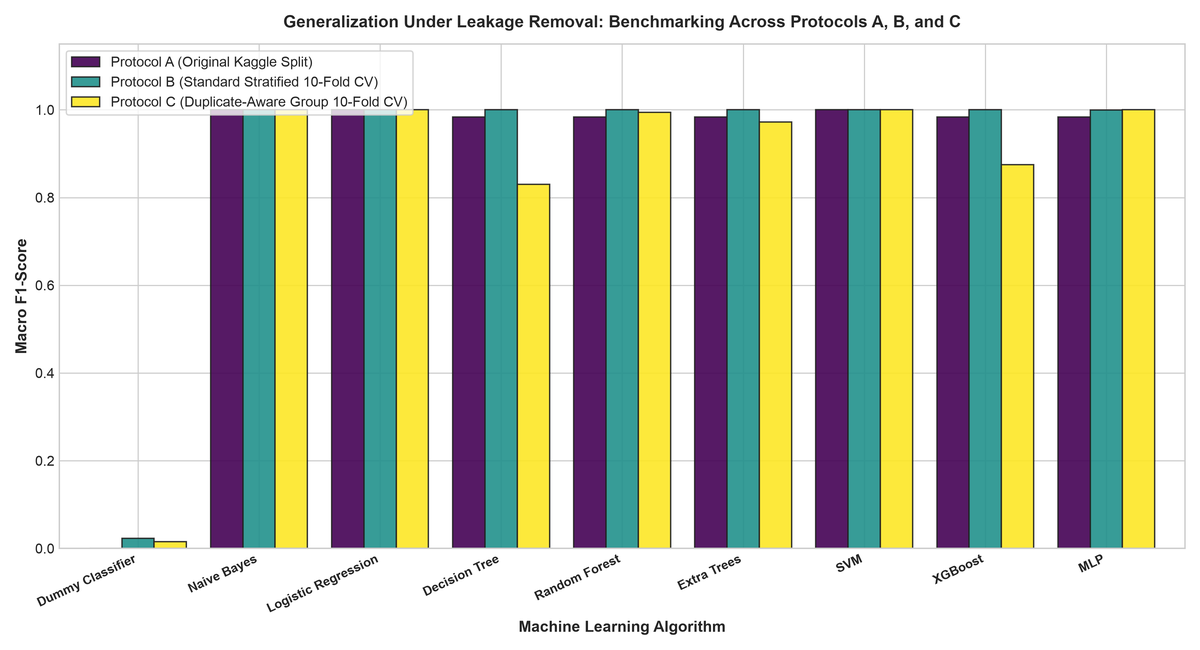
\includegraphics[width=0.9\textwidth]{protocol_comparison.png}
\caption{Cross-protocol performance comparison across the 9-model hierarchy. Notice the sharp degradation of Decision Tree and XGBoost under Protocol C.}
\label{fig:protocol_comparison}
\end{figure}

\begin{figure}[H]
\centering
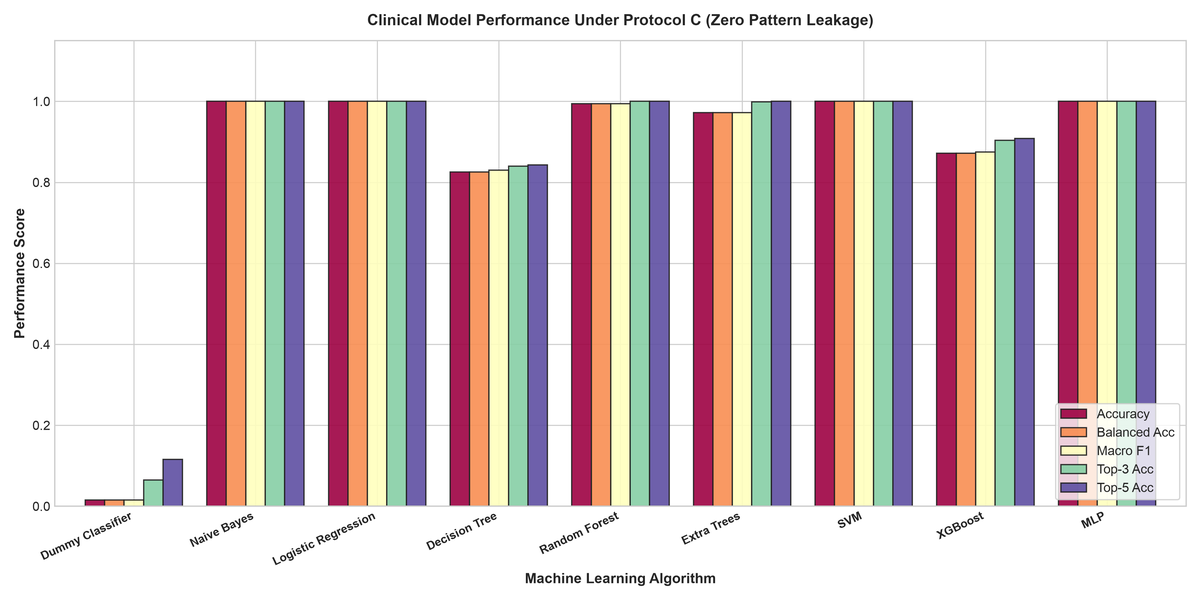
\includegraphics[width=0.9\textwidth]{model_performance.png}
\caption{Comprehensive metric breakdown under Protocol C (Zero Pattern Leakage), comparing Accuracy, Balanced Accuracy, Macro F1, Top-3, and Top-5 Accuracy.}
\label{fig:model_performance}
\end{figure}

% ==============================================================================
\section{Leakage-Aware Feature Selection and Dimensionality Reduction}
\label{sec:feature_selection}

To investigate whether multi-disease prediction requires all 132 symptoms or can operate on a compact clinical subset, we evaluated five feature-selection paradigms: Filter methods (Mutual Information, Chi-Square), Embedded methods ($L_1$-regularized Logistic Regression, Random Forest Gini importance), and Wrapper methods (Recursive Feature Elimination, RFE). Crucially, all feature ranking and selection procedures were fitted \emph{strictly inside each training fold} under Protocol C to prevent validation contamination.

\begin{table}[H]
\caption{Predictive Performance Across Feature Subsets ($k \in \{132, 100, 75, 50, 30, 20, 10\}$) Under Protocol C Across Model Families}
\label{tab:feature_selection_summary}
\centering
\scriptsize
\setlength{\tabcolsep}{2pt}
\begin{tabular}{cc|cccc|cccc|cccc}
\toprule
\multirow{2}{*}{\textbf{Method}} & \multirow{2}{*}{\textbf{$k$}} & \multicolumn{4}{c|}{\textbf{Logistic Regression}} & \multicolumn{4}{c|}{\textbf{MLP Neural Net}} & \multicolumn{4}{c}{\textbf{Random Forest}} \\
\cmidrule{3-14}
& & \textbf{Acc} & \textbf{F1} & \textbf{Top-3} & \textbf{Ret.} & \textbf{Acc} & \textbf{F1} & \textbf{Top-3} & \textbf{Ret.} & \textbf{Acc} & \textbf{F1} & \textbf{Top-3} & \textbf{Ret.} \\
\midrule
Full Baseline & 132 & 1.0000 & 1.0000 & 1.0000 & 100.0\% & 1.0000 & 1.0000 & 1.0000 & 100.0\% & 0.9939 & 0.9939 & 1.0000 & 100.0\% \\
\midrule
\multirow{6}{*}{Mutual Info}
& 100 & 0.9988 & 0.9988 & 1.0000 & 99.9\% & 0.9756 & 0.9765 & 0.9988 & 97.7\% & 0.9854 & 0.9854 & 0.9988 & 99.1\% \\
& 75  & 0.9939 & 0.9939 & 0.9988 & 99.4\% & 0.9610 & 0.9615 & 0.9976 & 96.2\% & 0.9817 & 0.9819 & 0.9988 & 98.8\% \\
& 50  & 0.9683 & 0.9687 & 0.9866 & \textbf{96.9\%}* & 0.9768 & 0.9773 & 0.9878 & \textbf{97.7\%}* & 0.9463 & 0.9471 & 0.9805 & \textbf{95.3\%}* \\
& 30  & 0.8354 & 0.8349 & 0.9585 & 83.5\% & 0.8415 & 0.8449 & 0.9476 & 84.5\% & 0.8098 & 0.8112 & 0.9512 & 81.6\% \\
& 20  & 0.7512 & 0.7520 & 0.9134 & 75.2\% & 0.7573 & 0.7567 & 0.9146 & 75.7\% & 0.7220 & 0.7237 & 0.8902 & 72.8\% \\
& 10  & 0.4329 & 0.4328 & 0.6707 & 43.3\% & 0.4415 & 0.4393 & 0.6585 & 43.9\% & 0.4329 & 0.4326 & 0.6500 & 43.5\% \\
\midrule
\multirow{6}{*}{$L_1$ Logistic}
& 100 & 0.9988 & 0.9988 & 1.0000 & 99.9\% & 0.9988 & 0.9988 & 1.0000 & 99.9\% & 0.9866 & 0.9866 & 1.0000 & 99.3\% \\
& 75  & 0.9939 & 0.9939 & 1.0000 & 99.4\% & 0.9829 & 0.9811 & 1.0000 & \textbf{98.1\%}* & 0.9793 & 0.9792 & 1.0000 & \textbf{98.5\%}* \\
& 50  & 0.9671 & 0.9671 & 0.9951 & \textbf{96.7\%}* & 0.9695 & 0.9702 & 0.9976 & \textbf{97.0\%}* & 0.9256 & 0.9263 & 0.9744 & 93.2\% \\
& 30  & 0.9110 & 0.9104 & 0.9805 & 91.0\% & 0.9293 & 0.9275 & 0.9866 & 92.8\% & 0.8915 & 0.8915 & 0.9659 & 89.7\% \\
& 20  & 0.8305 & 0.8313 & 0.9707 & 83.1\% & 0.8329 & 0.8438 & 0.9732 & 84.4\% & 0.8049 & 0.8052 & 0.9549 & 81.0\% \\
& 10  & 0.5280 & 0.5289 & 0.7976 & 52.9\% & 0.5317 & 0.5275 & 0.7768 & 52.8\% & 0.5098 & 0.5103 & 0.7610 & 51.3\% \\
\bottomrule
\end{tabular}
\vspace{2pt}
\par\noindent{\footnotesize *Meets the predefined operational retention criterion of $\ge 95.0\%$ retained Macro F1 relative to the 132-feature baseline. Ret. denotes Retained Macro-F1 percentage.}
\end{table}

\subsection{Smallest Subset Satisfying the \texorpdfstring{$\ge 95\%$}{>= 95\%} Retained Criterion}
\label{subsec:smallest_subset}
As documented in Table~\ref{tab:feature_selection_summary} and \cref{fig:feature_count_vs_f1}:
\begin{enumerate}
    \item Under both \textbf{Mutual Information} and \textbf{$L_1$ Logistic Regression}, \textbf{$k = 50$ symptoms} is the smallest feature subset that satisfies the predefined operational criterion of $\ge 95\%$ retained Macro-F1:
    \begin{itemize}
        \item Logistic Regression achieves \textbf{96.9\% retained F1} (F1: 0.9687, Top-3: 98.66\%) with Mutual Information.
        \item Multi-Layer Perceptron (MLP) achieves \textbf{97.7\% retained F1} (F1: 0.9773, Top-3: 98.78\%) with Mutual Information.
        \item Random Forest achieves \textbf{95.3\% retained F1} (F1: 0.9471, Top-3: 98.05\%) with Mutual Information.
    \end{itemize}
    \item We emphasize that the $\ge 95\%$ retained threshold is an \emph{operational benchmark threshold} defined for comparative evaluation, not clinical proof of exhaustive medical coverage.
\end{enumerate}

\begin{figure}[H]
\centering
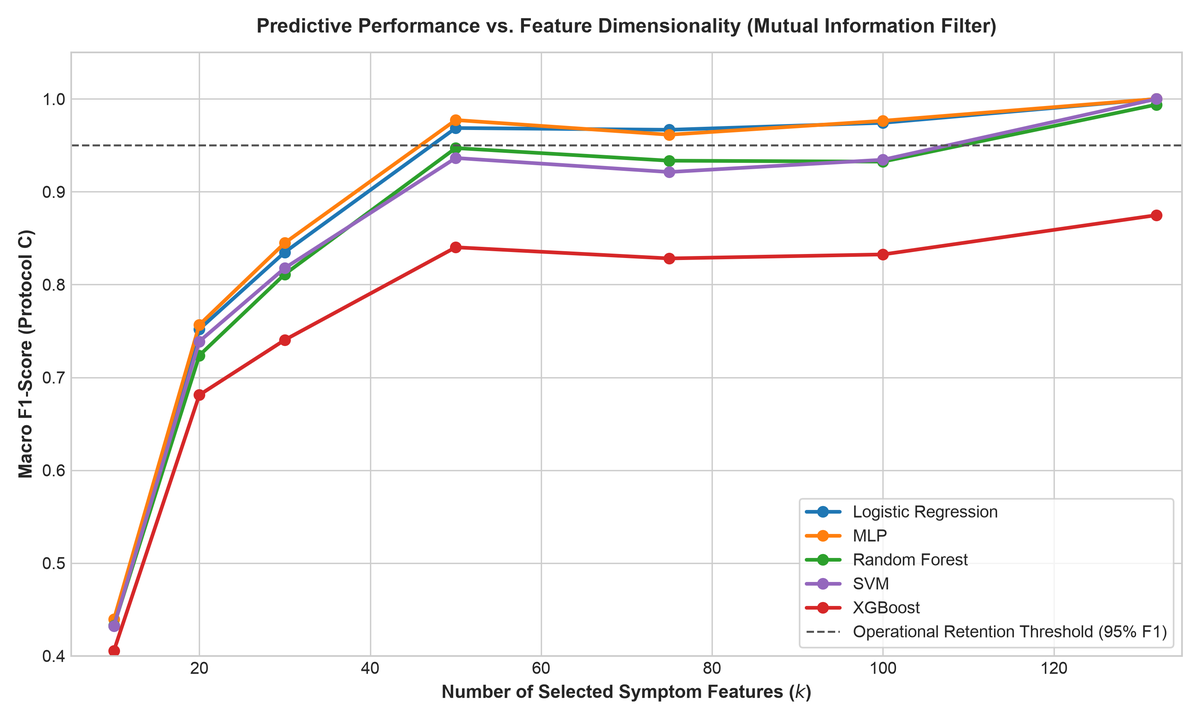
\includegraphics[width=0.9\textwidth]{feature_count_vs_macro_f1.png}
\caption{Macro F1-score as a function of symptom subset size ($k$) across models under Mutual Information feature selection. The dashed line marks the 95\% operational retention threshold.}
\label{fig:feature_count_vs_f1}
\end{figure}

\begin{figure}[H]
\centering
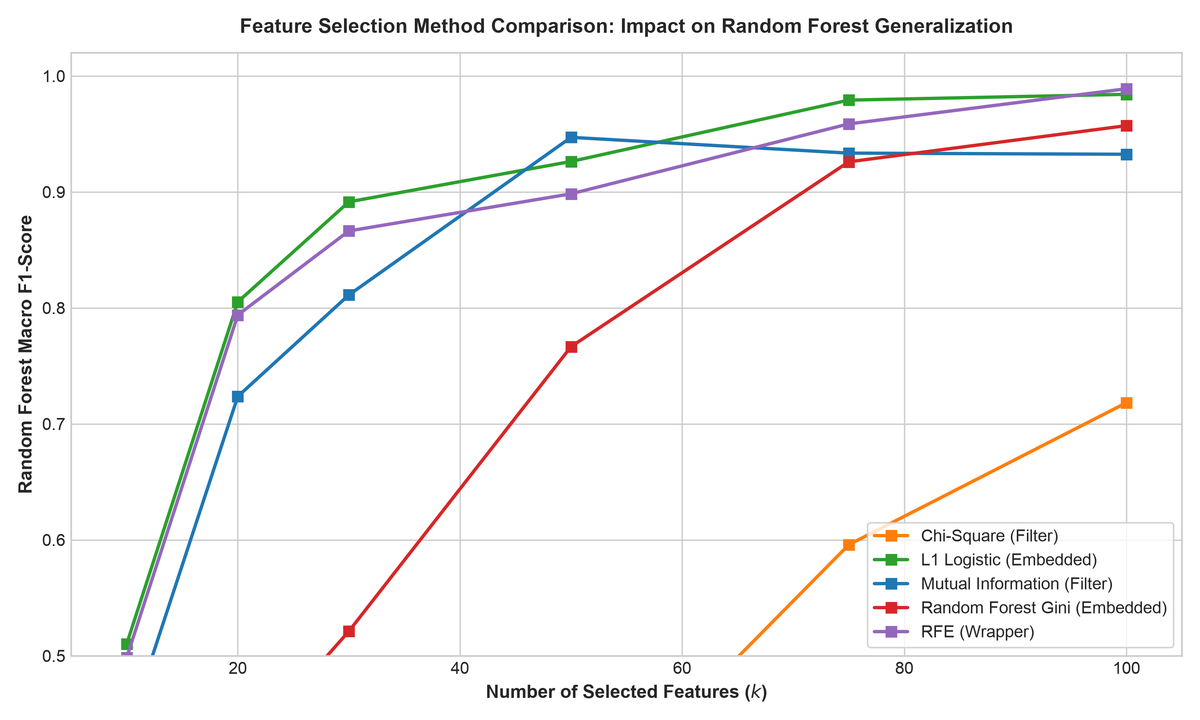
\includegraphics[width=0.9\textwidth]{feature_selection_comparison.png}
\caption{Feature selection method comparison on Random Forest under Protocol C. Notice the severe performance degradation of Chi-Square due to the suppression of high-information shared symptoms across overlapping diseases.}
\label{fig:feature_selection_comparison}
\end{figure}

\begin{figure}[H]
\centering
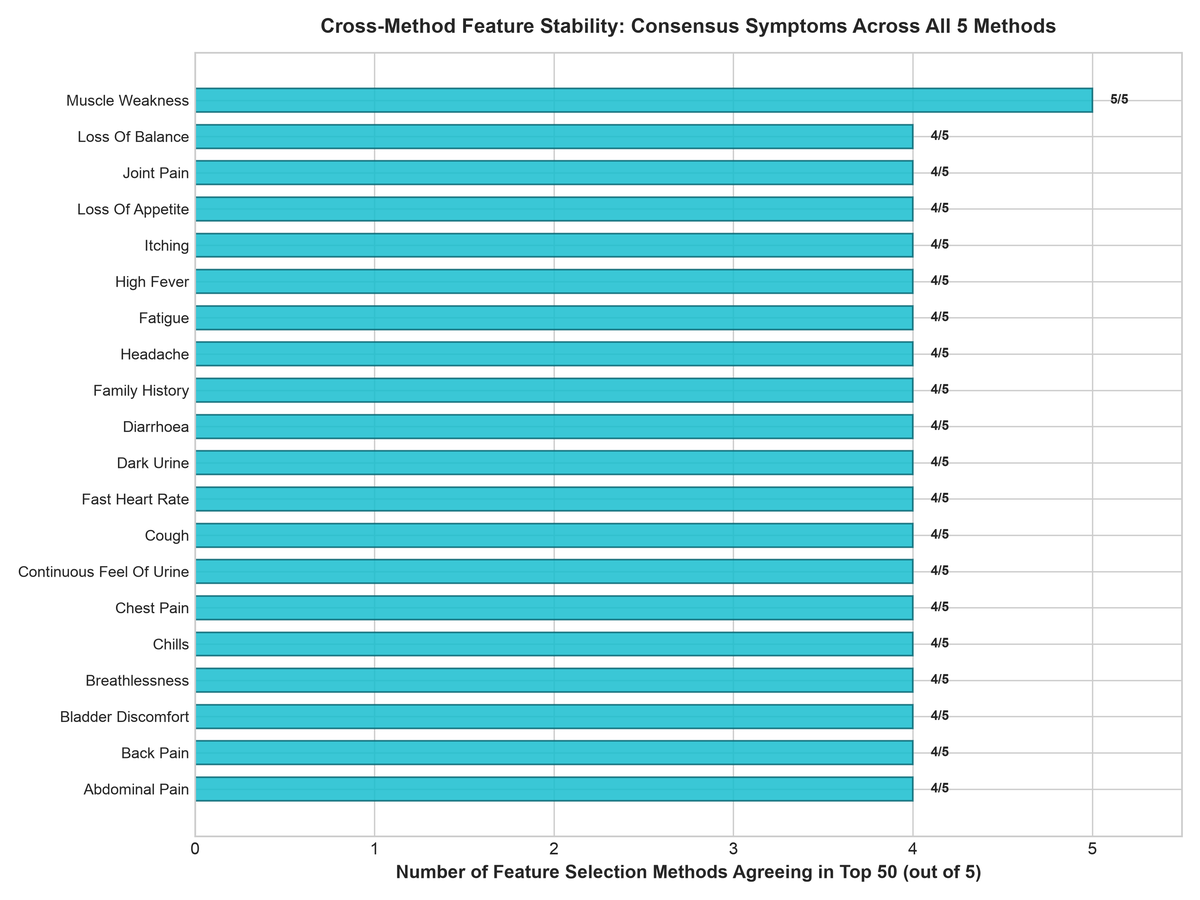
\includegraphics[width=0.9\textwidth]{feature_selection_stability.png}
\caption{Cross-method consensus: Top 20 symptoms identified consistently across independent feature selection methods within the top 50 ranked features.}
\label{fig:feature_selection_stability}
\end{figure}

\subsection{Differential Diagnosis Resilience at Aggressive Compression}
\label{subsec:differential_resilience}
When symptom dimensionality is aggressively reduced below $k=50$:
\begin{itemize}
    \item Under $L_1$ Logistic feature selection at \textbf{$k=30$ symptoms}, Top-1 Macro F1 declines to 0.9104, yet \textbf{Top-3 accuracy remains at 98.05\%} and \textbf{Top-5 accuracy reaches 99.02\%}.
    \item Even at \textbf{$k=20$ symptoms}, Top-3 accuracy is maintained at \textbf{97.07\%} and Top-5 accuracy at \textbf{98.29\%}.
    \item These results indicate that Top-$k$ evaluation can preserve substantially higher candidate-ranking performance than Top-1 classification under aggressive feature reduction.
\end{itemize}

\subsection{Empirical Analysis of Chi-Square Ranking Behavior}
\label{subsec:chisquare_analysis}
Under the duplicate-aware evaluation and feature-selection protocol used in this study, chi-square-based ranking produced substantially poorer predictive performance (declining to 71.4\% at $k=100$ and 35.4\% at $k=50$; \cref{fig:feature_selection_comparison}). A dataset-level audit revealed its ranking was strongly associated with symptom frequency and disease breadth ($r = -0.9069$ between $\chi^2$ score and prevalence):
\begin{enumerate}
    \item In a balanced 41-class cohort, binary symptoms occurring in only one disease achieve the maximum theoretical $\chi^2$ score ($\chi^2 = 4800.0$), ranking ultra-specific single-disease symptoms at the very top (20 symptoms covering only 9 of the 41 diseases).
    \item Conversely, high-information shared symptoms present across multiple conditions (e.g., \emph{vomiting} in 17 diseases, \emph{fatigue} in 17 diseases) received the lowest $\chi^2$ scores ($\chi^2 \approx 2704$).
    \item Because 32 of the 41 diseases lack exclusive private symptoms and depend primarily on combinations of shared symptoms, chi-square ranking stripped the models of the combinatorial features required to differentiate overlapping pathologies.
\end{enumerate}

\subsection{Feature Selection Stability Across Independent Folds}
\label{subsec:stability_folds}
To verify that the $k=50$ threshold does not reflect an artifact of a single lucky split, we audited selection stability across all 10 independent duplicate-aware folds:
\begin{itemize}
    \item For Mutual Information, the top 15 features exhibited \textbf{10/10 selection stability} across all 10 folds: \emph{fatigue, vomiting, high fever, loss of appetite, nausea, headache, abdominal pain, yellowish skin, yellowing of eyes, chills, skin rash, malaise, chest pain, joint pain,} and \emph{sweating}.
    \item For $L_1$ Logistic Regression, 15 symptoms also achieved 10/10 fold stability.
    \item Across all five independent feature-selection paradigms, 31 symptoms achieved $\ge 80\%$ cross-method consensus (\cref{fig:feature_selection_stability}), confirming that the compressed feature space captures clinically established core diagnostic indicators.
\end{itemize}
